% !TeX spellcheck = en_GB
\documentclass[10pt,a4paper]{article}
\usepackage[latin1]{inputenc}
\usepackage{color}
\usepackage{graphicx} %pictures
\usepackage{listings} %code
\usepackage{algorithm2e} %for psuedo code
%setup for code
\lstset{
tabsize=2, %indent
numbers=left,  % where to put the line-numbers
numbersep=5pt, % how far the line-numbers are from the code
}



\title{Finding the Convex Hull with Application to Distance Measurements for a Formula Student Car}
\author{Benedikt Schlereth}
\date{\today}

\begin{document}
	\maketitle
	\tableofcontents
	\pagebreak
	
	\begin{abstract}
	To find cones on the track for autonomous racing a computer has to visualize them and know how far away they are.
	For Visualizing the features of the cones inside the image are filtered out. After extracting the color the contours have rough edges. To smooth them out the convex hull gives back a nice contour with the out-most boundary of the cones. Knowing the dimension of the cone and proportions a Distance estimation can be done.
	\end{abstract}
	
	\section{Introduction}
	Formula-Student is an international design and construction competition where teams from all around the world are constructing and then racing single seat formula racecars. With	the new event of Formula Student Driver less Teams are encouraged to develop their own self Driving cars.
	My motivation is to kick off the develpment of our own Driverless Vehicle by implementing the first step and provididing a way to detect the boundaries of a race track.
	The track markings are strictly defined in the rules for the competition. It is important to know that the left border of the track is marked with small blue cones and the right one with small yellow cones. 
	Start, finish and timekeeping lines are marked with big orange cones. It is also important to know, that the maximum distance between two cones in driving direction is 5m but in corners it can be expected to be less \cite{handbook}. Knowing the rules is important to understand the track-layout and be able to make an estimation on how far ahead a self-driving-vehicle needs detect boundaries. 
	
	\section{Steps to extract the Features}
	To find the cones inside a picture one could create a dataset of 100+ cones and then train a neural network. But working with a neural network brings the additional difficulties to choose a network type that is efficient to run on a mobile platform while being reliable.
	It is also not necessary for this type of application to detect different objects in one frame.
	With only cones in three different colors to detect it is quite simple to describe the features of them.
	To visualize the process i choose a scene with green cones an different lighting and ground.
	\begin{figure}[h]
		\centering
		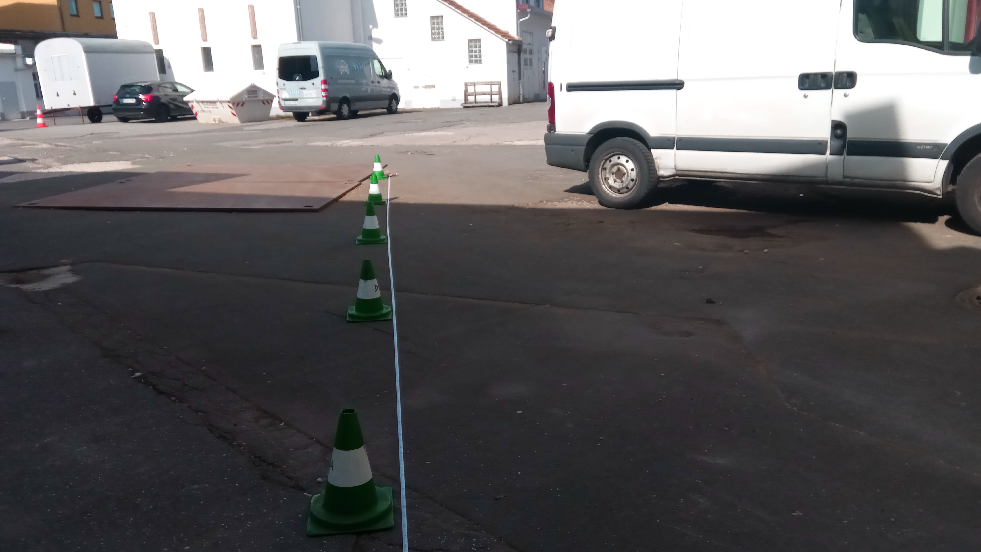
\includegraphics[width=0.5\textwidth]{Abb/start.png}
		\caption{example image}
		\label{example image}
	\end{figure}
	The picture is taken from a height of $1,2 m$ and the distance between the cones is $2m$ with the nearest $2m$ and the farthest $10m$ away from the camera. The resolution is 1920 by 1080 pixel. The resolution is choosen in a way that a CMOS camera can deliver 30 fps.
	 
	\subsection{color filtering}
	The most obvious feature is the color. So the first step is to implement a colorfilter.
	\begin{lstlisting}[language=Python]
hsv = cv2.cvtColor(image, cv2.COLOR_BGR2HSV)
	
# value for colorfilter
lower_green = np.array([30, 100, 0])
upper_green = np.array([90, 255, 255])
	
mask = cv2.inRange(hsv, lower_green, upper_green)
res = cv2.bitwise_and(hsv, hsv, mask=mask)

blur = cv2.GaussianBlur(res, (15, 15), 0)
return blur, mask
	\end{lstlisting}
	The image provided for the colorfilter needs to be converted from the RGB values to the HSV colorspace.
	The HSV describes the color not with an eight-Bit value for red, green and blue but with a circle where the first value is for the color with 0 beeing red and 255 blue.
	The second value is needed for the saturation and the third and last value describes how bright the color will be represented.
	
	With knowing how the HSV-colorspace works it is possible to find the right values which will describe the color of our cones. It will be necessary to try the colorfilter for images in bright sunlight as well as cloudy conditions the make sure to be able to detect cones in every possible environment.
	
	Next up is comparing every Pixel with our given value. With the OpenCV function "inRange" one image will be read and compared to our boundaries. It returns a binary image which means everywhere the color was in Range a one is remaining and everywhere else a zero.
	
	\subsection{Contours}
	After the Color-filter we are left with a binary image. Now it is quit easy to detect the edges of where it changes from black to white.
	
	\begin{figure}[h]
		\centering
		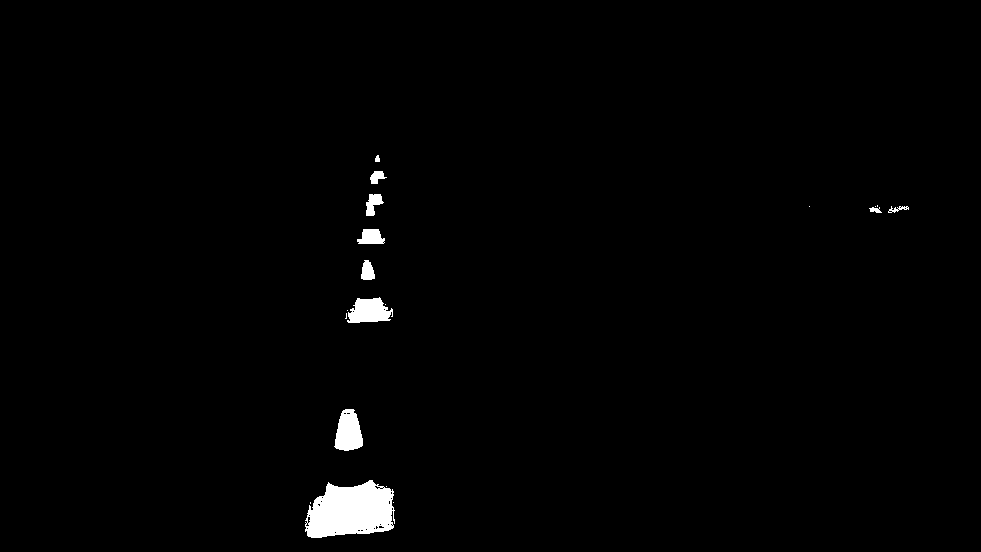
\includegraphics[width=0.5\textwidth]{Abb/mask.png}
		\caption{binary-image}
		\label{binary-image}
	\end{figure}
	
	But as seen in the top right hand corner of the image some noise will be left inside the picture. Therefore another filter is needed. A good difference between important and noisy areas is the size of the contour. This will delete all small contours which are most probably not important but also cones that are far away. The first test showed that excluding such cones does not matter.
	
	\subsection{Hierarchy}
	Sometimes small dots or areas are left inside the contours which make up the cones. Luckily the contour-function gives us back the hierarchy of each contours. By filtering out the parts lying inside of bigger areas leaves only parts of the cones with no noise inside the contour.
	
	\subsection{Convex-hull}
	The next step will be to find the convex hulls. What those are and how they are found will be described in the section \ref{convex-hull}. The convex-hull leaves a very good approximation of the cones edges as seen in Figure \ref{convex-hull-picture}
	\begin{figure}[h]
		\centering
		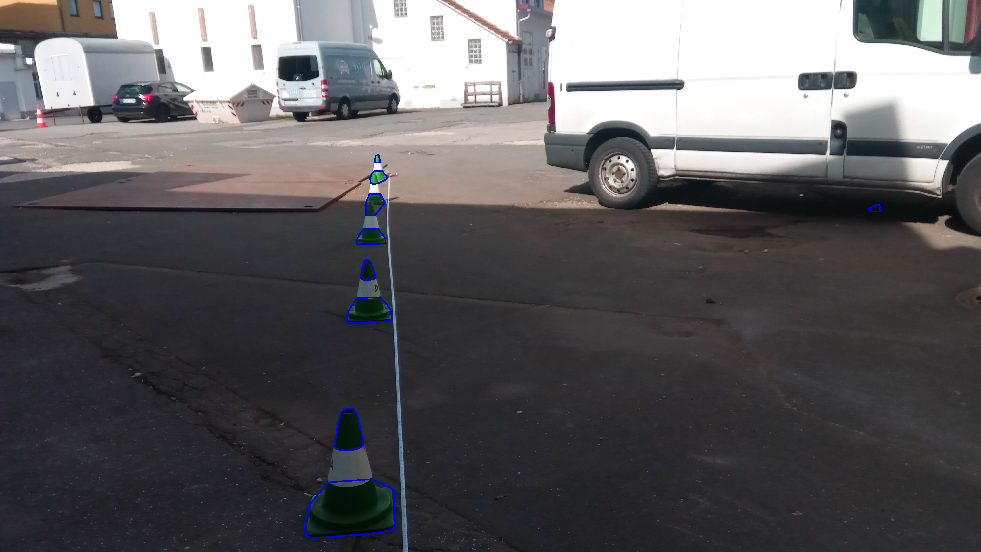
\includegraphics[width=0.5\textwidth]{Abb/convex-hull.png}
		\caption{convex-hull}
		\label{convex-hull-picture}
	\end{figure}
	
	\subsection{Aspect ratio}
	A nice feature of the cones is the round top part. So no matter at what angle or distance the convex hull is detected the ratio between the height and width stays the same. With this Feature extracted know all top parts of the cones should be detected. As seen in the picture \ref{top-part} not all cones can be detected. It is more important to accurately detect real cones and not detect an object in the middle of the track.
	\begin{figure}[h]
		\centering
		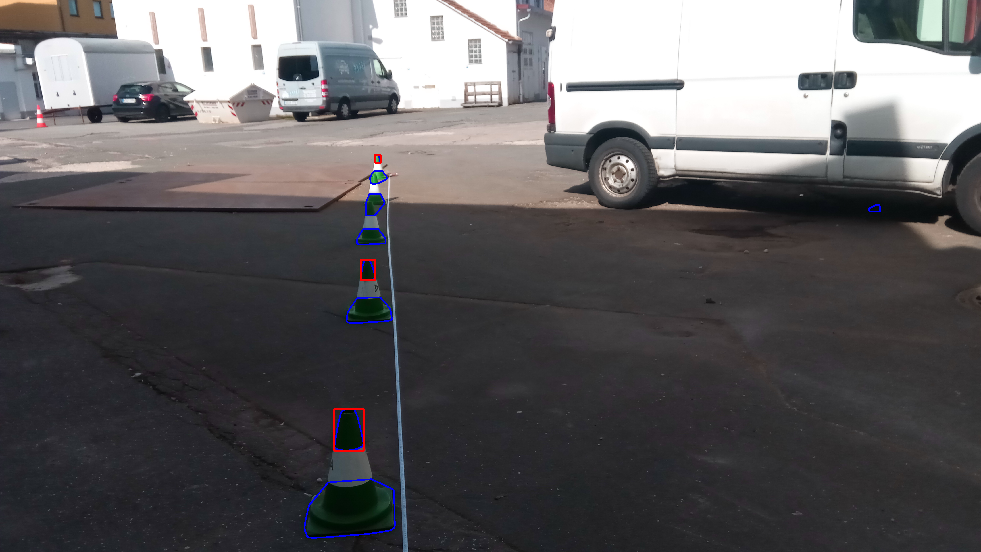
\includegraphics[width=0.5\textwidth]{Abb/top_part_cone.png}
		\caption{top-part}
		\label{top-part}
	\end{figure}
	
	
	\subsection{Bounding box}
	With every top part of the cones found now the bottom part needs to be added. Therefore the distance to every other contour is calculated and the nearest one below the top part belongs to the same cone.
	The maximum points of both contours give the outlines of a bounding box which is drawn with red-color in Figure \ref{bounding-box}
	
	\begin{figure}[h]
		\centering
		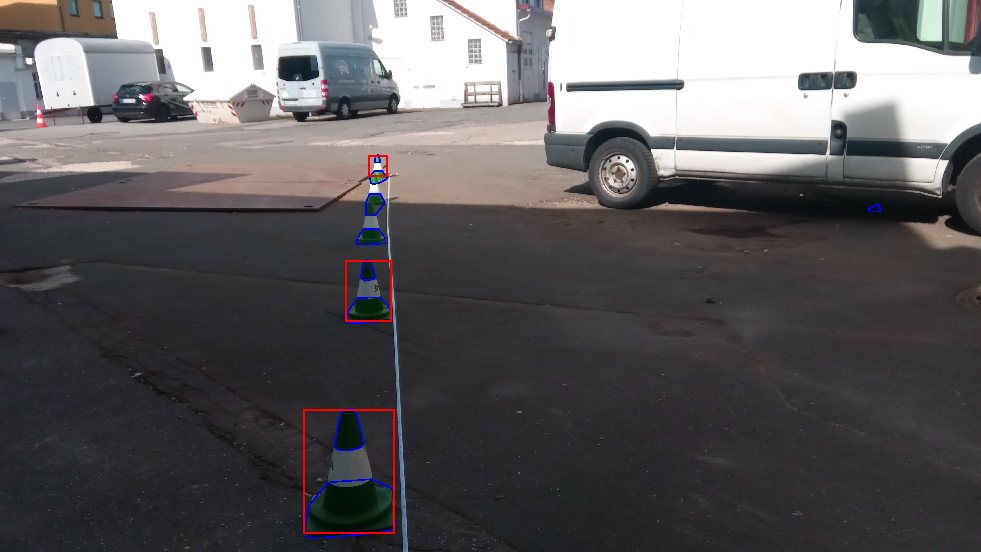
\includegraphics[width=0.5\textwidth]{Abb/bounding-box.png}
		\caption{bounding-box}
		\label{bounding-box}
	\end{figure}
	
	\section{Convex-Hull algorithm by Graham} \label{convex-hull}
	The Convex Hull is the smallest region containing all points while having no Concave corners.
	
	\section{Distance estimation}
	To find out where the cones are on the track the distance to each cone must be calculated. 
	With only one camera the number of pixel is the only value that can be used. It is also important to know the resolution of the used camera.
	While it is quit simple to take high-resolution pictures and the wait for a computer to analyze it, it is not so easy in a real-time application. To make sure the picture can be read and analyzed the input will be limited to an 1920x1080 image which can be processed by a small computer-module like a Jetson-Nano in a reasonable frame-rate of about 30 fps.
	A stereo camera on the other hand would make triangulation possible.

	\subsection{Height} \label{height-estimation}
	% estimate the distance with the pixel in vertical direction 
	The numbers of pixel measuring the y-Height($h$) can be used to estimate the distance ($D$) to each cone. With the bounding box function of OpenCV it is quite easy to get the height. 
	\begin{figure}[h]
		\centering
		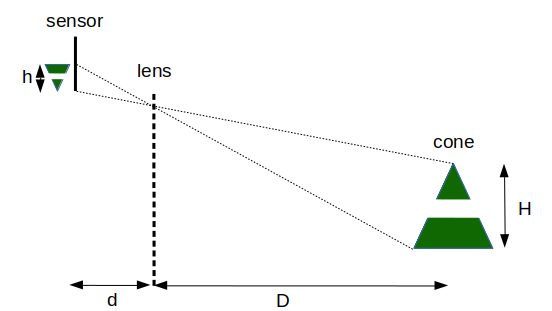
\includegraphics[width=0.5\textwidth]{Abb/distance-estimation.png}
		\caption{distance-estimation}
		\label{distance-estimation}
	\end{figure}
	The thin lens equation is given as
	$$\frac{D}{H}=\frac{d}{h}$$
	where $d$ is an unknown variable depending on the manufacturer of the camera.
	$d$ can than be calculated with $d=\frac{D_1*h_1}{H}$ and then calibrated by taking a picture of a cone at a known distance. After evaluating the dimensions a good estimation for $\frac{D_1}{h_1}$ is $440\frac{m}{px}$.
	So to calculate the distance to each cone the following equation can be used:
	$$D = \frac{440}{h}$$
	
	\subsection{Side-Length}
	% estimate distance with the distance between the top and bottom part of the cone
	The top part of a cone is round and so no matter at what angle the camera is detecting the cone, the proportions are the same. If the foot is detected it can make a difference for the distance estimation. Therefore it is possibly a better feature for evaluating the distance.
	By using the side-length $s$ as seen in Figure \ref{corners} for the distance estimation it can be valid for all angles of the cone.
	
	\begin{figure}[h]
		\centering
		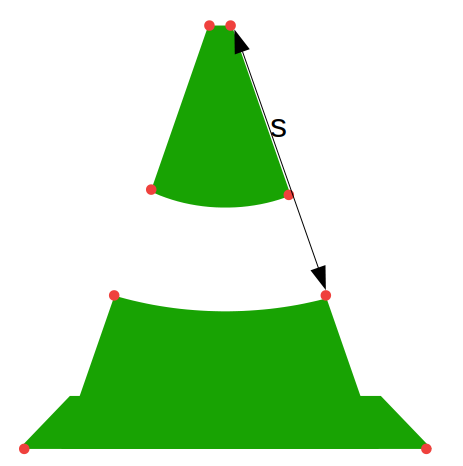
\includegraphics[width=0.5\textwidth]{Abb/corners.png}
		\caption{corners of a cone}
		\label{corners}
	\end{figure}
	
	To measure the side-length the corner points need to be found first. Inside of Figure \ref{corners} the important points are marked with red-dots.
	For all cases it can be estimated that the cone will have a flat point on the top and therefore both parts of the cone are trapezium-shaped.
	The algorithm \ref{extreme-points} returns good corner points for cones standing upright. This code has to be run for the top section as well es the bottom section of the cone to be able to find all 8 corners.

	\begin{algorithm}
		\KwIn{convex-hull}
		\KwOut{extrem-points}
		find bounding Box\;
		get top-line\; 
		get bottom-line\;
		\While{point in convex hull}
			{\uIf{$y_{point} = y_{top-line}$}
				{\uIf{$x_{point} \le x_{left-top-corner}$}
					{left-top-corner = point;}
				\uIf{$x_{point} \ge x_{right-top-corner}$}
					{right-top-corner = point;}
				}
			\uIf{$y_{point} = y_{bottom-line}$}
				{\uIf{$x_{point} \le x_{left-bottom-corner}$}
					{left-bottom-corner = point;}
				\uIf{$x_{point} \ge x_{right-bottom-corner}$}
					{right-bottom-corner = point;}
			}
		}
	\label{extreme-points}
	\caption{extreme-points} 
	\end{algorithm}

	 
	By drawing a bounding box around one section the area where the top and bottom corner-points should lie can be estimated. Next step is to go through the points of the convex hull. If it lies inside a margin of the top or bottom line of the bounding box it is maybe a corner point. So the next step is then to look if it lies more to the left or to the right then an already scanned point. That way the outermost points will be detected.
	 
	By then calculating the distance between the Top-Right-corner of the top part to the Top-Right-corner of the bottom part the side-length of the cone can be calculated and used for a distance estimation similar to the one used in section \ref{height-estimation} with the calibrated value for $\frac{D_1}{h_1}=280\frac{m}{px}$
	$$D=\frac{280}{s}$$
	
	
	\subsection{Error}
	% estimate the error of the calculation
	\subsubsection{rotation}
	As discussed earlier it is important to estimate the distance at every possible angle the cone is facing the car. One example picture was taken to show what kind of error can occur with detecting the wrong height.
	
	\subsubsection{Pixel-Error}
	To make sure the track can be monitored correctly it is important to know how good the distance estimation will be. By using only the number of pixel for an estimation you need to know how accurate the size can be estimated and how big the difference is for one pixel.
	\begin{figure}[h]
		\centering
		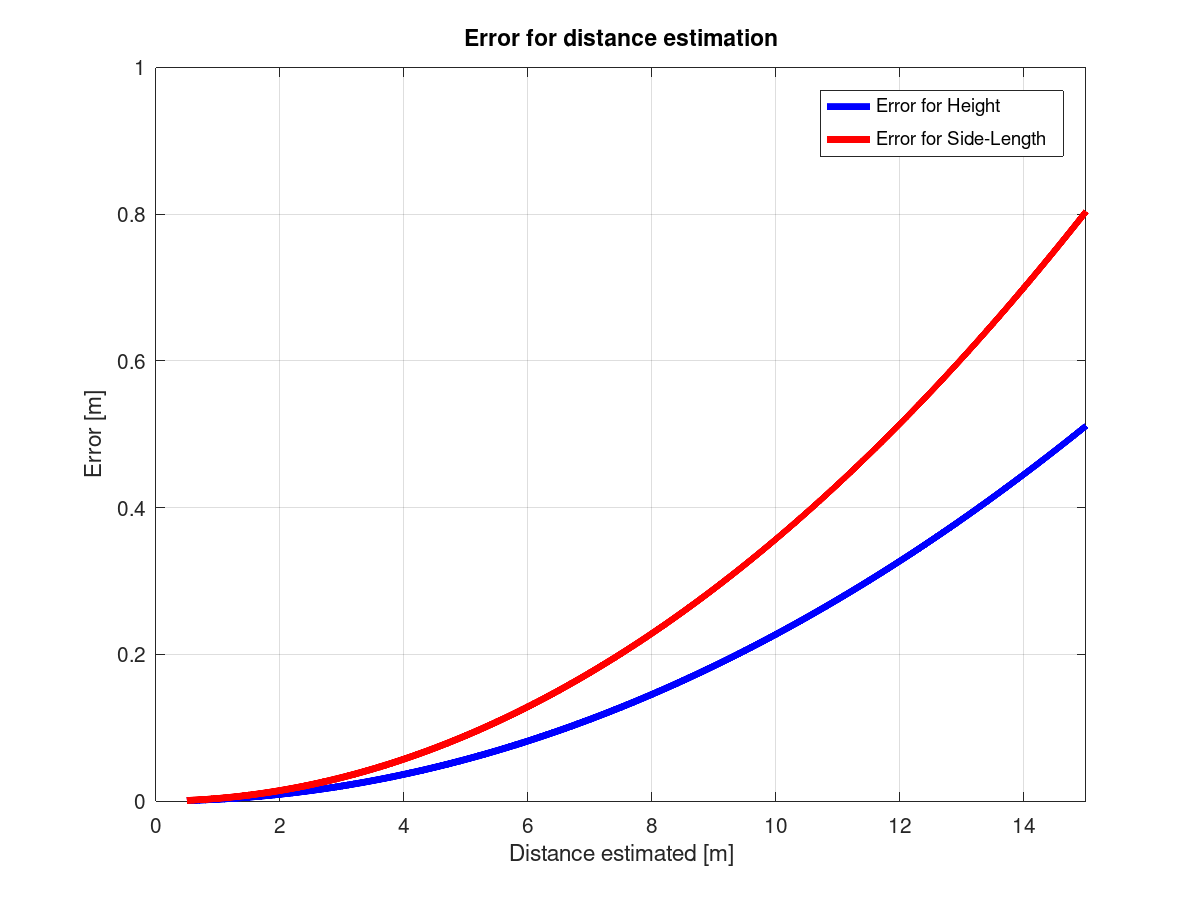
\includegraphics[width=0.7\textwidth]{Abb/pixel-error.png}
		\caption{error for one pixel}
		\label{error-pixel}
	\end{figure}
	
	\subsection{Disruption}
	% discuss possible disruptions that can occur while driving (e.g bumps on the track)
	The most discouraging dial to get right will be the color-filter. It has to more or less accurately detect the right color inside the image. While in use it must not detect any yellow banners or the blue sky as cones, while working in bright sunlight as well as pouring rain.
	
	An often seen "DNF" (Did not Finish) in the driverless class is often detecting tipping over cones in one round and not being able to complete the track on the next round due to a imperfect course. So hopefully by detecting only the upstanding cones the ones not marking the true edge of the track wont disturb the car.
	
	\section{Tests}
	% test the algorithmus with different lighting and roadcondition
	
	\section{Summary}
	% Discussion after evaluating the tests
	
	\section{Discussion}
	% Steps in the future (e.g draw own pictures to test faulty inputs, test robustness of code)
	\section{reference}
	
	\begin{thebibliography}{xxxxxxxxxxxxxxxxxxx}
		\bibitem[convex-hull, 1983]{convex-hull}{Finding the Convex Hull of a Simple Polygon, Ronald L. Graham, F.Frances Yao, 1983}
		\bibitem[FSG-Handbook,2020]{handbook}{FSG Competition Handbook 2020}
		\bibitem[opencv, 2019]{opencv}{Sunila Gollapudi, Learn Computer Vision Using OpenCV, 2019}
	\end{thebibliography}
\end{document}